\setcounter{page}{1}
\section{Zielsetzung}
Ziel dieses Versuchs ist die Bestimmung der Magnetfelder unterschiedlicher Spulen.
\section{Theorie}
 Bewegte elektrische Ladungen erzeugen Magnetfelder.
 Die entstehenden Feldlinien sind immer geschlossen und verlaufen senkrecht zum Stromfluss.
 Die Magnetfeldstärke $\overrightarrow{H}$ eines stromdurchflossenen Drahtes
 kann mit dem Biot-Savart-Gesetz
 \begin{equation}
   d\overrightarrow{B} = \frac{\mu_{0}I\cdot \overrightarrow{ds} \times
   \overrightarrow{r}}{4 \pi r^3}
 \end{equation}
 bestimmt werden.
 Dabei ist $\mu_0$ die Magnetische Feldkonstante mit einem Wert von
 $4\pi \cdot 10^{-7}\, \frac{V \cdot s}{A\cdot m}$ und $r = |\overrightarrow{r}|$, also
 \begin{equation*}
   r = \sqrt{x^2 +y^2 +z^2} \,.
 \end{equation*}
Die Magnetische Flussdichte einer langen stromdurchflossenen Spule wird durch die Formel
\begin{equation}
  \overrightarrow{B}= \mu_r \mu_0 \cdot \frac{n}{l}\cdot I
  \label{eqn:2}
\end{equation}
berechnet.
Dabei beschreibt $l$ die Länge der Spule und $n$ die Windungszahl.
$\mu_r$ beschreibt die Permeabilität eines Stoffes,
der in das Spuleninnere gebracht wird, um ein Magnetfeld zu verstärken.
Zum Beispiel ist die Permeabilität des Ferromagneten Eisen bis zu 5000.
Ferromagnetische Stoffe können magnetisiert werden und werden zum Magneten,
wenn sie mit einem in Kontakt kommen.
Dies geschieht, weil sich die Elementarmagnete alle
in die selbe Richtung ausrichten.\cite{on1}\\
Wird nun ein Magnetfeld an eine (Ring-)Spule mit einem ferromagnetischen Kern gelegt,
entsteht eine Hysteresekure, wie sie in Abbildung (\ref{fig:hys1}) zu sehen ist.
%http://www.ulfkonrad.de/physik/groessen/mag_stoffe.htm
\begin{figure}[H]
\centering
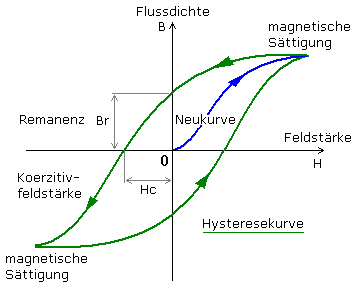
\includegraphics[scale=0.8]{hysteresekurve.png}
\caption{Hysteresekurve\protect\cite{on2}}
\label{fig:hys1}
\end{figure}

%http://elektroniktutor.de/elektrophysik/magkurve.html
Die charakteristischen Eigenschaften einer Hysteresekurve,
wobei die Flussdichte $B$ gegen die äußere Feldstärke $H$ augetragren wird, sind im folgenden aufgezählt.
\begin{enumerate}
  \item Neukurve:\\
  Die Neukurve beschreibt den erstmaligen Anstieg der Flussdichte bei Erhöhung des angelegten Stroms.
  \item Sättigungspunkte:\\
  Ab einer gewissen Feldstärke, bleibt die Flussdichte konstant.
  Dieser Wert wird als magnetische Sättigung bezeichnet.
  Die Sättigungsunkte sind in negativer und positiver Richtung betragsmäßig gleich.
  \item Remanenzflussdichte:\\
  Die Remanenzflussdichte ist der Schnittpunt mit der y-Achse.
  Sie beschreibt das bestehenbleibende Magnetfeld, wenn kein Strom fließt.
  Dabei gilt, dass der Wert des Schnittpunktes in (+y)-Richtung gleich dem Wert des Schnittpunktes in (-y)-Richtung ist.
  \item Koerzitivkraft :\\
  Die Koerzitivkraft beschreibt den Schnittpunkt mit der x-Achse.
  Sie ist ein Maß für die magnetische Feldstärke,
  die benötigt wird um den entstehenden "Restmagnetismus" zu beseitigen\cite{on3}
\end{enumerate}
%http://www.itwissen.info/Koerzitivkraft-K-coercive-force.html
Bei einem Helmholzspulenpaar ist das Magnetfeld abhängig vom Unterschied zwischen dem Radius $r$
und dem Abstand $d$. Liegt der Unterschied bei $d=2\cdot x$ wird für das Feld in der Mitte der
Helmholtz-Spule ein allgemeiner Fall betrachtet.
Haben die Helmholzspulen einen geringen Abstand, so ist das Feld im Inneren wie eine kurze Spule zu betrachten.

\begin{equation}
  B(0) = B_1(x) + B_1(-x) = \frac{\mu_0\cdot I\cdot R^2}{(R^2+x^2)^{3/2}}
  \label{eqn:3}
\end{equation}
Dabei ist $\mu_0$ die magnetische Flussdichte und R der Spulenredius.
